\documentclass{article}
\usepackage{graphicx}
\usepackage{physics}
\usepackage{amsmath}
\graphicspath{ {C:/Users/Peter/Desktop/} }
 
\usepackage[utf8]{inputenc}
\usepackage[T1]{fontenc}

\usepackage[german]{babel}
\begin{document}
\title{RISE weltweit Erfahrungsbericht - Optical Eigenmodes an der Universit{\"a}t St Andrews}
\author{ Peter Manshausen}
\date{19. September 2017}
\maketitle
\pagebreak
\renewcommand\contentsname{Inhalt}
\tableofcontents
\section{Allgemeiner Teil}
\subsection{Einleitung}
Meine Berwerbung f\"{u}r das Projekt folgte einer Empfehlung eines Freundes aus meinem Wohnheim, der mich auf das Programm aufmerksam machte. Auch wenn ich noch nicht so recht wusste, was ich in den Sommerferien so vorhaben w\"{u}rde -- zum Bewerbungstermin sind diese immerhin noch mehr als ein halbes Jahr entfernt -- suchte ich mir drei Projekte heraus. Dieses spezielle in St Andrews interessierte mich besonders, weil die unterliegenden Konzepte (Elektrodynamik, Eigenbasen, Simulation) auch in meinem Studium gerade aktuell waren. So hoffte ich darauf, das Erlernte auch einmal anwenden zu k\"{o}nnen. Ich wurde nicht entt\"{a}uscht. Aber auch in anderer Hinsicht war die Zeit in Schottland sehr lohnend und ich kann das RISE-Programm w\"{a}rmstens weiterempfehlen.
\subsection{Vorbereitung und Organisation}
Der wichtigste Punkt, um den man sich k{\"u}mmern sollte, sobald man die Zusage vom DAAD erhalten hat, ist die Unterkunft. Die Uni vermietet prinzipiell nur bis einschlie{\ss}lich der letzten Augustwoche, da danach die Zimmer gewartet warden und dann die regul{\"a}ren Studenten zur{\"u}ckkehren. F\"{u}ndig wird man meiner Erfahrung nach weniger \"{u}ber einschl{\"a}gige Websites, die dem deutschen \emph{WG gesucht} vergleichbar w{\"a}ren, sondern eher \"{u}ber Facebookgruppen, insbesondere \emph{Find Accommodation for Next Year}. Ausserdem kann man es \"{u}ber die \emph{Stipnetz St Andrews} Gruppe versuchen – dort war ich erfolgreich. Preislich muss man sich auf Mieten ab 400{\pounds} einstellen, wenn man in der Stadt selbst wohnen will, Preise bis 550{\pounds} sind die Regel. Billiger wird es, wenn man in Dundee oder einem der umliegenden D{\"o}rfer bleibt, dann muss man jedoch t{\"a}glich den Weg mit dem Bus auf sich nehmen.  
\subsection{Schottland allgemein}
Ich kann nur dringend empfehlen, sich vor oder nach dem Praktikum noch etwas Zeit zu nehmen, um den Rest Schottlands zu erkunden. W\"{a}hrend Ziele wie Loch Ness, Fort William oder Glasgow auf der Karte nah aussehen, hat man mit Bus und Bahn von St Andrews aus kaum eine Chance, \"{u}bers Wochenende weiter wegzufahren. Schon ins 50 km entfernte Edinburgh braucht man zwei Stunden. Ich hatte vor dem Praktikum noch eine Woche Zeit und war je drei Tage auf dem West Highland Way wandern und auf dem Edinburgh Fringe Festival. Beides ist sehr zu empfehlen und das Fringe Festival sollte man auf jeden Fall terminm\"{a}ssig auf dem Schirm haben. So viel Auswahl an Musicals, Theaterst\"{u}cken, Comedy-Auftritten und Konzerten bekommt man sonst nirgends, allein hier k\"{o}nnte man eine ganze Woche verbringen. F\"{u}r mehrt\"{a}gige Wandertouren durch die tolle Highland-Landschaft ist zu empfehlen, sich fr\"{u}h ($>$2 Wochen) um Unterk\"{u}nfte auf dem Weg zu bem\"{u}hen, Juli und August sind Hochsaison. Andererseits ist es auch sehr reizvoll, ein Zelt mitzunehmen, denn in Schottland gilt Jedermannsrecht. Unbedingt mitnehmen sollte man dann wasserdichte Wanderschuhe und Jacke. Das britische Wetter wurde w\"{a}hrend meines Aufenthalts seinem Ruf definitif gerecht, ich h\"{a}tte statt der kurzen Hose besser einen Pullover mehr eingepackt.
\subsection{St Andrews und Umgebung}
St Andrews ist eine nette Kleinstadt am Meer voller (Golf-)Touristen und -- w\"{a}hrend des Semesters -- Studenten. Die (Ruine der) Kathedrale, die alten Universit\"{a}tsgeb\"{a}ude wie St Salvator's College und die (Ruine der) Burg kann man gut auf einem ausgedehnten Spaziergang erkunden. Ausserdem lohnt es sich, einmal den idyllischen Lade Braes Walk entlangzulaufen, der an einem Bach entlang durch die Stadt geht. St Andrews ist nat\"{u}rlich besonders f\"{u}r den riesigen Golfplatz bekannt, auf dem man auch gut eine Runde joggen kann, wenn man kein Golf spielt. In der n\"{a}heren Umgebung von St Andrews ist der Fife Coastal Path, ein Wanderweg, der immer an der K\"{u}ste entlang geht. Es empfiehlt sich zum Beispiel an einem Wochenende von St Andrews Richtung S\"{u}den nach Crail oder bis Anstruther zu wandern, dort zu \"{u}bernachten (in Anstruther gibt es ein Hostel) und dann am Sonntag mit dem Boot auf die Isle of May zu fahren. In die Highlands (bspw. den Cairngorms National Park) f\"{a}hrt man \"{u}ber Leuchars mit Bus und Bahn auch f\"{u}r eine Tageswanderung. Die anderen Praktikanten und ich haben so zum Beispiel Beinn Mheadhonach bei Blair Atholl erwandert. Die Uni pr\"{a}gt die Stadt nat\"{u}rlich ungemein und die alten College-Geb\"{a}ude lohnen einen Besuch. \"{U}berrascht hat mich die starke Fokussierung der Forschungst\"{a}tigkeiten der Physikalischen Fakult\"{a}t: Geforscht wird hier insbesondere an Astronomie, Photonik und Festk\"{o}rperphysik. Andere grosse Forschungsthemen wie Teilchen- oder Umweltphysik scheinen schwach oder garnicht vertreten zu sein.
\subsection{Freizeitgestaltung}
In St Andrews selbst ist zwischen den Semestern nicht sonderlich viel los, da die allermeisten Studenten verreist sind und nur die \"{u}brigbleiben, die an ihren Abschlussarbeiten schreiben, also die meiste Zeit in der Bibliothek verbringen. Die meisten Einrichtungen bleiben jedoch offen, darunter die Anlagen des Hochschulsports und die Student Union Bar auf St Marys Pl. F\"{u}r mich war das Angebot des Hochschulsports nicht sehr lohnend, weil man ohne Studenten- oder Bedienstetenstatus jeden Kurs bzw. jede Nutzung der Angebote wie Schwimmbad oder Kraftraum einzeln bezahlen muss. Stattdessen habe ich mich bei Functional Fitness St Andrews angemeldet, einem privaten Fitnessstudio, wo es t\"{a}glich Fitness-Kurse gibt, insbesondere zwischen 17:00 und 20:00. Besonders hilfreich fand ich die Excel-Tabelle mit Kontaktdaten der anderen RISE-Stipendiaten. Zusammen sind wir mehrfach abends in den Pub gegangen oder haben am Wochenende Ausfl\"{u}ge in die Umgebung gemacht.
\section{Fachlicher Teil}
\subsection{Einf\"{u}hrung}
Mein Projekt in St Andrews stand unter dem Titel "Higher Order Optical Eigenmodes". Es war damit theoretisch-numerischer Natur. Grundlegend geht es darum, wie man die Ausbreitung von Licht in Medien beschreiben kann, in denen die Polarisation $P$ der Konstituentenmolek\"{u}le nicht linear von der Feldst\"{a}rke des elektromagnetischen Feldes abh\"{a}ngt.Stattdessen k\"{o}nnen wir schreiben
\begin{equation}
P= \epsilon_0 (\chi^{(1)}\textbf{E}+\chi^{(2)}\textbf{EE}+ \chi^{(3)}\textbf{EEE}+\mathcal{O}(\textbf{E}^4))
\end{equation}
F\"{u}r lineare Effekte (also wenn nur $\chi^{(1)}$ ungleich null) ist es m\"{o}glich, eine Basis von Eigenfunktionen zu Operatoren wie Energiedichte, Intensit\"{a}t oder Strahlbreite zu finden. In dieser Basis nehmen die Operatoren analog zur Quantenmechanik Diagonalform an und man kann die entsprechenden Observablen mit einer bestimmten \"{U}berlagerung maximieren oder minimieren. Dr. Mazilus Gruppe ist es so beispielsweise gelungen, die nat\"{u}rliche Beugungsgrenze zu durchbrechen, also einen Strahl st\"{a}rker zu fokussieren als durch die Beugungsgrenze vorhergesagt (vgl. Baumgartl, 2011). Ein \"{a}hnliches Verfahren soll auch f\"{u}r Interaktionen h\"{o}herer Ordnung gefunden werden. Einer der einfachsten nichtlinearen Effekte ist das sogenannte Three Wave Mixing, bei dem zwei Lichtstrahlen interagieren und einen dritten erzeugen.
\begin{figure}[h]
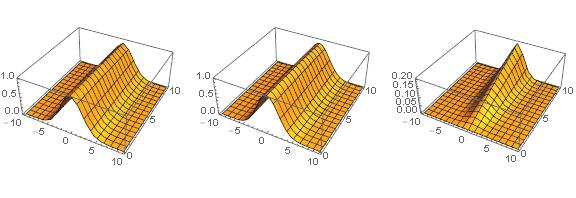
\includegraphics[width=\textwidth]{TWM}
\caption{Ein Beispiel f\"{u}r Three Wave Mixing - man sieht die Felder links und in der Mitte, die relativ konstant bleiben und das dritte Feld, das ganz rechts durch die Interaktion entsteht. Man beachte die unterschiedlichen Gr\"{o}ssenordnungen der beiden urspr\"{u}nglichen und des entstehenden Feldes (alle Einheiten beliebig).}
\end{figure}
Dies macht man sich beispielsweise im allt\"{a}glichen gr\"{u}nen Laserpointer zunutze, in dem zwei Infrarot-Wellenz\"{u}ge einen Wellenzug doppelter Frequenz hervorbringen. Die Interaktion passiert aber nicht nur im Frequenz-,
sondern \\ auch im Ortsraum. Die Frage, der ich nachgegangen bin, ist, ob es Konfigurationen des r\"{a}umlichen Feldinputs gibt, sodass dieser nach einer gewissen Ausbreitungsdistanz (der sog. Interaktionsl\"{a}nge) reproduziert wird. Dies w\"{a}re "nahe dran" an einer Eigenfunktion.
\subsection{Modellierung}
F\"{u}r die Betrachtung des Three Wave Mixing wurde ein Modell eines zweidimensionalen optischen Kristalls in Mathematica beschrieben. Dieser Kristall ist also praktisch eine Ebene, deren eine Richtung die Ausbreitungsrichtung (longitudinal) und deren andere die Transversalrichtung ist, welche die Form des Strahls bestimmt. Dazu machte ich mich in der ersten Woche zun\"{a}chst mit Mathematica vertraut und simulierte einfachere Versionen, zum Beispiel in einer Dimension. Verwendet wurde die Mathematica-Funktion NDSolve zur schrittweisen numerischen Approximation der L\"{o}sung der Differentialgleichungen (s. u.) Eine einfache Simulation des Three Wave Mixing zeigt Abb. 1: Licht breitet sich nach schr\"{a}g rechts hinten aus und der Strahl hat dabei je nach x-Koordinate (um Null herum) eine unterschiedliche Intensit\"{a}t, die durch die H\"{o}he (zwischen Null und Eins f\"{u}r die ersten beiden Felder) dargestellt wird. Das Verhalten der Felder wird beschrieben durch drei gekoppelte partielle Differentialgleichungen, die Manley-Rowe-Gleichungen (vgl. New, 2011). Diese k\"{o}nnen aus den grundlegenden Maxwell-Gleichungen der Elektrodynamik abgeleitet werden. Es ist
\begin{equation}
\frac{\partial E_1} {\partial z}=-\frac{i}{2k_1} \pdv [2]{E_1}{x}-\frac{i \omega_1}{2 c n_1} \chi^{(2)}E_3 E_2^*e^{-i\Delta k z}
\end{equation}
\begin{equation}
\frac{\partial E_2} {\partial z}=-\frac{i}{2k_2} \pdv [2]{E_2}{x}-\frac{i \omega_2}{2 c n_2} \chi^{(2)}E_3 E_1^*e^{-i\Delta k z}
\end{equation}
\begin{equation}
\frac{\partial E_3} {\partial z}=-\frac{i}{2k_3} \pdv [2]{E_3}{x}-\frac{i \omega_3}{2 c n_3} \chi^{(2)}E_1 E_2 e^{i\Delta k z}
\end{equation}
wobei $E_i$ die Felder mit Frequenzen $\omega_i$, Wellenzahlen $k_i$ und Brechungsindizes $n_i$ sind, $z$ die Ausbreitungs- und $x$ die Transversalrichtung und $\chi^{(2)}$ der Suszeptibilit\"{a}tstensor zweiter Ordnung. Dieser gibt also die St\"{a}rke der Kopplung der Felder an. F\"{u}r den Exponentialterm gilt $\Delta k= k_3-k_2-k_1$, die Frequenzen sind \"{u}ber $\omega_3=\omega_1+\omega_2$ verbunden.
 Ein wichtiger Test, um zu pr\"{u}fen, ob das Computermodell funktioniert, ist die Energieerhaltung, die man aus den Manley-Rowe-Gleichungen auch analytisch herleiten kann (umgekehrt nahmen Manley und Rowe die Energieerhaltung urspr\"{u}nglich an, um die Relationen zu gewinnen). Abb. 2 zeigt einen Plot, in dem man ablesen kann, dass auch bei sich \"{a}nderndem Verh\"{a}ltnis der Felder die Gesamtenergie erhalten bleibt. 
\begin{figure}[h]
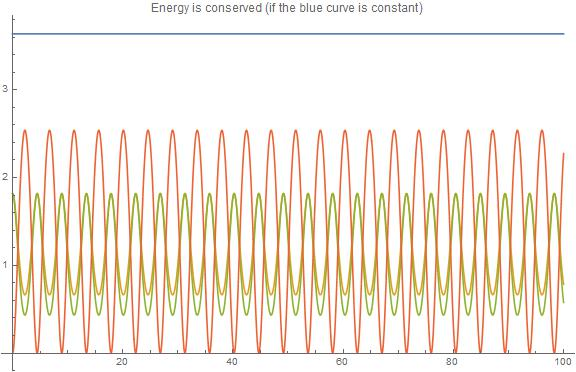
\includegraphics[scale=0.4]{energyconservation}
\caption{Energieerhaltung: Die blaue Linie oben zeigt den Verlauf der Gesamtenergie (konstant) w\"{a}hrend die Absolutbetr\"{a}ge der einzelnen Felder (restliche Kurven) periodisch variieren. Alle Einheiten beliebig.}
\end{figure}
\subsection{Mein Projekt}
Ein ganz \"{a}hnliches Modell hatte in dieser Gruppe schon ein Student namens Liam Gallagher f\"{u}r seine Masterarbeit genutzt und mit einer Basis aus -- in x-Richtung -- Hermite-Gauss-f\"{o}rmigen Strahlen den Input-Output-Tensor konstruiert. Ich habe diese Arbeit weitergef\"{u}hrt und verallgemeinert, indem statt reflektierender Randbedingungen ($E(0)=E(x_{max})=0$) periodische Randbedingungen zugelassen wurden  ($E(0)=E(x_{max})$). Dazu wurde dann eine Basis aus Fouriermoden der Form 
$$E_i(z)= \sum_{n=-N}^{N} a_{i,n}(z) \exp(n \frac{2\pi x}{x_{max}})$$
verwendet. Dadurch wird die Frage nach der Form der Outputfunktion zur Frage nach der Gr\"{o}sse der Koeffizienten $a_{i,n}(z)$. Sie lautet nun, ob es Felder gibt, die nach einer bestimmten Ausbreitungsl\"{a}nge wieder dieselben (oder \"{a}hnliche) Fourierk\"{o}ffizienten haben, wie am Anfang. Einsetzen in die Manley-Rowe-Relations (2)-(4) liefert zun\"{a}chst
\begin{equation}
k_1 i\frac{\partial a_{1, n}} {\partial z}=\frac{1}{2}(\frac{n 2 \pi}{x_{max}})^2 a_{1, n}-\frac{\chi^{(2)} \omega_1^2}{c^2}  e^{-i\Delta k z} \sum_{m=-N}^{N} a_{2, m}^* a_{3, n+m}
\end{equation}
\begin{equation}
k_2 i\frac{\partial a_{2, n}} {\partial z}=\frac{1}{2}(\frac{n 2 \pi}{x_{max}})^2 a_{2, n}-\frac{\chi^{(2)} \omega_2^2}{c^2} e^{-i\Delta k z} \sum_{m=-N}^{N} a_{1, m}^* a_{3, n+m} 
\end{equation}
\begin{equation}
k_3 i\frac{\partial a_{3, n}} {\partial z}=\frac{1}{2}(\frac{n 2 \pi}{x_{max}})^2 a_{3, n}-\frac{\chi^{(2)} \omega_3^2}{c^2} e^{i\Delta k z} \sum_{m=-N}^{N} a_{1, m} a_{2, n-m}. 
\end{equation}
Dabei ist besonders eindr\"{u}cklich, dass der Multiplikationsterm in einen Faltungsterm \"{u}bergeht (die Summe am Ende der Gleichungen), wie vom Faltungstheorem vorhergesagt. An der Form der Gleichungen ist abzulesen, dass eine Symmetrie bez\"{u}glich der komplexen Phase der Koeffizienten besteht. Die Gleichungen sind invariant unter der Transformation 
$$a_{1, n} \longrightarrow a_{1, n} \exp(i \phi_1)$$
$$a_{2, n} \longrightarrow a_{2, n} \exp(i \phi_2)$$
$$a_{1, n} \longrightarrow a_{3, n} \exp(i \phi_3)$$
$$wobei \ \phi_3=\phi_1+\phi_2.$$
Gesucht sind demnach nicht unbedingt Koeffizienten, die \emph{genau} die anf\"{a}nglichen reproduzieren, es sind jeweils unabh\"{a}ngige Phasen f\"{u}r Feld eins und zwei erlaubt, die aber zusammen diejenige von Feld drei ergeben m\"{u}ssen. Mit dieser Bedingung l\"{a}sst sich eine Funktion $f$ definieren, welche die relevante Abweichung misst:

\begin{align}
\nonumber f(z)=\sum_{i=1}^{3}\bigg(\sum_{n} (\abs{a_{i, n}(z)} -\abs{a_{i, n}(0)})^2+(\bigl|\sum_n a_{i, n}(z) a_{i, n}^*(0) \bigr|-\sum_n\abs{ a_{i, n}(z) a_{i, n}^*(0)})^2\bigg) \\ +\ (\Im(a_{1,1}(z) a_{2,1}(z) a_{3,1}^*(z))-\Im(a_{1,1}(0) a_{2,1}(0) a_{3,1}^*(0)))^2
\end{align}
Dabei pr\"{u}ft der erste Term, der quadriert wird, ob die Absolutbetr\"{a}ge der Koeffizienten gleich sind, der zweite, ob innerhalb eines Feldes die Phase der Koeffizienten \"{u}bereinstimmt und der dritte, ob die Phasen der Felder eins und zwei zusammen die Phase des dritten Feldes ergibt. Da alle Beitr\"{a}ge nichtnegativ sind, verschwindet die Funktion $f(z)$ dann und nur dann, wenn jeder Beitrag null ist.

\subsection{Ergebnisse}
Tats\"{a}chlich beobachtet man exakte Periodizit\"{a}t geringer Periodenl\"{a}nge (auf der Skala der Periode des Absolutbetrags) genau f\"{u}r Konfigurationen, in denen die Felder des Inputs jeweils nur aus einer einzigen Fouriermode bestehen. In diesem Fall reproduzieren sich die Anfangsbedingungen bis auf die numerische Ungenauigkeit der L\"{o}sungsfunktion. Je mehr Fouriermoden hinzugef\"{u}gt werden, desto gr\"{o}sser ist die Interaktionsl\"{a}nge, nach der man ann\"{a}hernde Nullstellen der Fehlerfuktion $f(z)$ findet. Dies ergibt insofern Sinn, als wir Periodizit\"{a}ten f\"{u}r jeden einzelnen Koeffizienten erhalten, die Fehlerfunktin aber nur dann verschwindet, wenn \emph{alle} Periodenl\"{a}ngen an einem Punkt zusammenfallen. In dieser vereinfachten Betrachtung w\"{a}re die Interaktionsl\"{a}nge einfach das Kleinste Gemeinsame Vielfache der einzelnen Periodenl\"{a}ngen. Durch die Nichtlinearit\"{a}t ergeben sich jedoch noch zus\"{a}tzliche (einh\"{u}llende) Schwingungen, die ebenfalls mit den anderen zusammenfallen m\"{u}ssen. Dies reproduziert sehr gut die Ergebnisse des Doktoranden in meiner Arbeitsgruppe, der sich dem Problem aus einer etwas anderen Richtung n\"{a}hert (n\"{a}mlich ohne den Input von vornherein in eine Basis zu zerlegen), die ihn auf Diopantinische Gleichungen f\"{u}r die Periodenl\"{a}nge gef\"{u}hrt haben. Abb. 3 zeigt den Verlauf der Fehlerfunktion f\"{u}r die F\"{a}lle von je einer, zwei und drei Fouriermoden in den Feldern eins und zwei. Das dritte Feld ist am Anfang identisch null.
\begin{figure}[h]
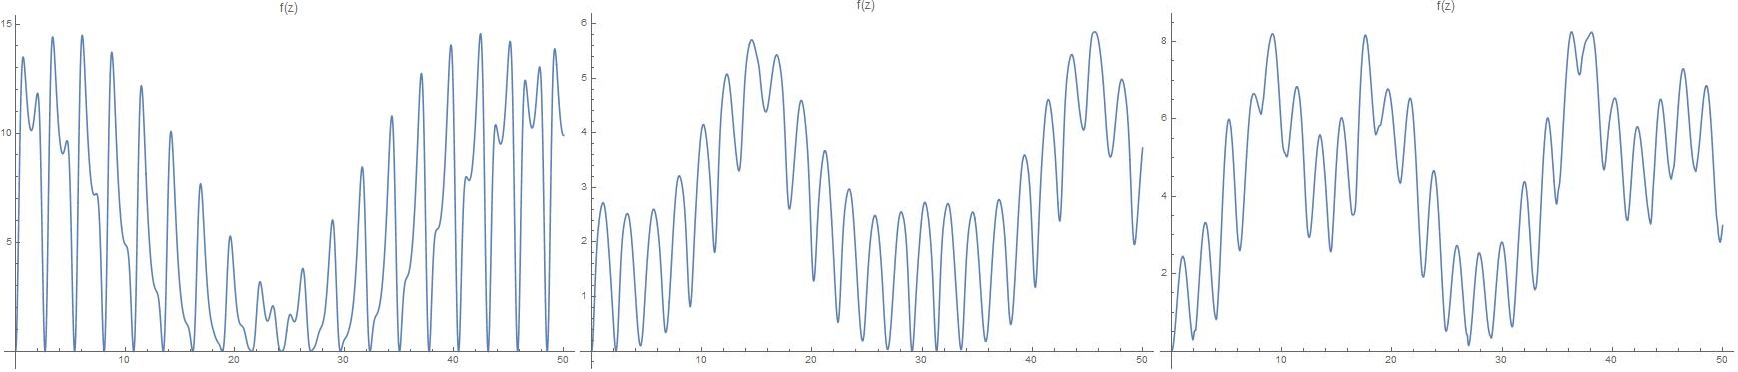
\includegraphics[width=\textwidth]{allthree}
\caption{Fehlerfunktion: Von links nach rechts mit Input von einer, zwei und drei Fouriermoden, die gaussf\"{o}rmig verteilt sind. Alle Einheiten beliebig.}
\end{figure}
Einen Einfluss auf die Interaktionsl\"{a}nge, so sie denn erkennbar ist, hat insbesondere der Wert der nichtlinearen Suszeptibilit\"{a}t $\chi^{(2)}$. So ist die Interaktionsl\"{a}nge ungef\"{a}hr invers proportional zu $\chi^{(2)}$, was Sinn ergibt, wenn man sich vor Augen f\"{u}hrt, dass dieser Wert die St\"{a}rke der Nichtlinearit\"{a}t und damit der Interaktion zwischen den Feldern wiedergibt. 
\subsubsection{Beispiel}
Zur Illustration betrachten wir den folgenden Input: Moden in $E_1$: $n=4 \ und\ 5$ und $E_2$: $n=3\ und \ 4$, L\"{a}nge des Kristalls in $x$-Rtg.: 10, L\"{a}nge des Kristalls in Propagationsrichtung $z$: 100, Frequenzen $\omega_1=\omega_2=5$, Brechungsindizes $n_1=n_2=1,5$, $n_3=1,6$. Dies entspricht dem mittleren Bild in Abb. 3. Numerisch finden wir eine vielversprechende Nullstelle der Funktion bei $z=31,3109$. Die Koeffizienten dort sind in der folgenden Tabelle aufgetragen.
\begin{center}
 \begin{tabular}{||c c c c||} 
 \hline
Feld & Fouriermode n & Absolutbetrag & Input-Absolutbetrag \\ [0.5ex] 
 \hline\hline
 1 & 4 & 0.78 &  0.78 \\ 
 \hline
 1 & 5 & 0.78 &  0.78 \\
 \hline
 2 & 3 & 0.78 &  0.78 \\
 \hline
 2 & 4 & 0.78 &  0.78 \\
 \hline
 3 & 7 & 0.01 &  0.00 \\
 \hline
 3 & 8 & 0.01 &  0.00 \\
 \hline
 3 & 9 & 0.01 &  0.00 \\ [1ex] 
 \hline
\end{tabular}
\end{center}
Der Absolutbetrag wird also gut reproduziert. Die Fehlerfunktion sorgt ebenfalls f\"{u}r eine Reproduktion der Phase, auf deren Darstellung ich hier jedoch verzichtet habe.
\subsection{Schlussfolgerung, offene Fragen und weitere Schritte}
Die Ergebnisse zeigen, dass der Ansatz des Zerlegens in Fouriermoden vielversprechend ist, eine gr\"{o}ssere Zahl dieser das System jedoch chaotisch macht. Daher w\"{a}re es sinnvoll, die Untersuchung des Systems mit nur einer einzelnen komplexen Exponentialfunktion als Profil weiterzuf\"{u}hren. Hier zeigt sich gerade der Kern des Problems: W\"{a}hrend Fourierentwicklung normalerweise erlaubt, jede Welle beziehungsweise jeden Koeffizienten einzeln anzuscha\"{u}n und zu entwickeln, funktioniert dies hier nicht, da das Problem nichtlinear ist und die Wellen sich daher nicht einfach (additiv) \"{u}berlagern, sondern gegenseititg beeinflussen. Mit einzelnen Moden k\"{o}nnte man zun\"{a}chst \"{u}berpr\"{u}fen, welche Rolle die Systemparameter $\chi^{(2)}, \omega_i, \Delta k, n_i$ spielen und dann dazu \"{u}bergehen, nicht eine Interaktionsl\"{a}nge zu suchen, nach der ein gegebener Input sich reproduziert, sondern bei gegebener L\"{a}nge des Kristalls nach demjenigen Input suchen, der nach dieser Propagationsdistanz wiederkehrt. Das w\"{a}re dann noch ein St\"{u}ck n\"{a}her an einer echten Eigenfunktion.
\subsection{Pers\"{o}nliche Einordnung}
Das Projekt war eine sehr lohnenswerte Erfahung, insbesondere, da mir \"{u}berraschend viele Anwendungen des Erlernten aus den Kursen an der Uni begegnet sind. Bei manchen recht abstrakt-mathematischen Lerninhalten wie Faltungen oder Zahlentheorie hatte ich mich schon gefragt, warum das \"{u}berhaupt wichtig ist. Diese Frage wurde im Laufe des Praktikums beantwortet. Ausserdem habe ich w\"{a}hrend des Praktikums den Umgang mit der Simulationssoftware Mathematica und dem Textverarbeitungssystem \LaTeX gelernt. Der Austausch mit den anderen Mitgliedern des Teams war sehr hilfreich.  Dabei h\"{a}tte ich mir teilweise etwas n\"{a}here Betreuung gew\"{u}nscht - gerade den Projektleiter Dr. Mazilu habe ich nur etwa w\"{o}chentlich getroffen, da er in der Zeit sehr besch\"{a}ftigt mit einer Konferenz und der Ver\"{o}ffentlichung eines Papers war. Dies hat mich andererseits dazu gebracht, unabh\"{a}ngiger zu arbeiten und mit Problemen nicht auf die Hilfe anderer zu warten, sondern sie selbst zu l\"{o}sen. Ausserdem konnte ich mich mit Fragen immer an Dr. Mazilus Promovenden Graeme wenden, dem ich sehr dankbar bin. Insofern kann ich sagen, dass mich das Praktikum auf viele Arten weitergebracht hat und ich es nur herzlich weiterempfehlen kann. F\"{u}r die M\"{o}glichkeit es durchzuf\"{u}hren m\"{o}chte ich dem DAAD und Dr. Mazilu ganz herzlich danken.
\section{Quellen, Literatur, Links}
\begin{itemize}
  \item Baumgartl, J. et al: Far Field subwavelength focusing using optical Eigenmodes, \emph{Applied Physics Letters}, vol. 98, 2011
  \item New, G.: Introduction to Nonlinear Optics, Cambridge University Press, 2011
  \item Boyd, R.: Nonlinear Optics, Third Edition, Elsevier, 2009
  \item Link zu meinem GitHub-Account, wo die Mathematica-Notebooks gespeichert sind, die ich verwendet habe: https://github.com/ManshaP/Internship-Optical-Eigenmodes
\end{itemize}

\end{document}